\lstdefinelanguage{json}{
    basicstyle=\normalfont\ttfamily,
    numbers=left,
    numberstyle=\scriptsize,
    stepnumber=1,
    numbersep=8pt,
    showstringspaces=false,
    breaklines=true,
    frame=lines,
    backgroundcolor=\color{background},
    literate=
     *{0}{{{\color{numb}0}}}{1}
      {1}{{{\color{numb}1}}}{1}
      {2}{{{\color{numb}2}}}{1}
      {3}{{{\color{numb}3}}}{1}
      {4}{{{\color{numb}4}}}{1}
      {5}{{{\color{numb}5}}}{1}
      {6}{{{\color{numb}6}}}{1}
      {7}{{{\color{numb}7}}}{1}
      {8}{{{\color{numb}8}}}{1}
      {9}{{{\color{numb}9}}}{1}
      {:}{{{\color{punct}{:}}}}{1}
      {,}{{{\color{punct}{,}}}}{1}
      {\{}{{{\color{delim}{\{}}}}{1}
      {\}}{{{\color{delim}{\}}}}}{1}
      {[}{{{\color{delim}{[}}}}{1}
      {]}{{{\color{delim}{]}}}}{1},
}

\chapter{Design di Dettaglio}
\label{chap:detailed-design}
In questo capitolo verrà illustrata l'organizzazione del codice per i componenti dell'architettura, i pattern utilizzati e le principali scelte implementative.

\section{Pattern utilizzati}
Sia per quanto riguarda l'architettura della parte client (simulatore e backend) che per quella della Mixed Reality è stato implementato il pattern MVC (\textit{Model}-\textit{View}-\textit{Controller}). Il pattern è composto da tre componenti principali:

\begin{itemize}
    \item \textbf{Model}: incapsula i dati, il recupero e la persistenza di questi nelle varie sorgenti;
    \item \textbf{View}: si occupa della presentazione dei dati all'utente;
    \item \textbf{Controller}: contiene tutta la business logic dell'applicazione, elaborando l'input dell'utente, recuperando e aggiornando le informazioni nel model.
\end{itemize}

\begin{wrapfigure}{r}{0.4\textwidth}
    \centering
    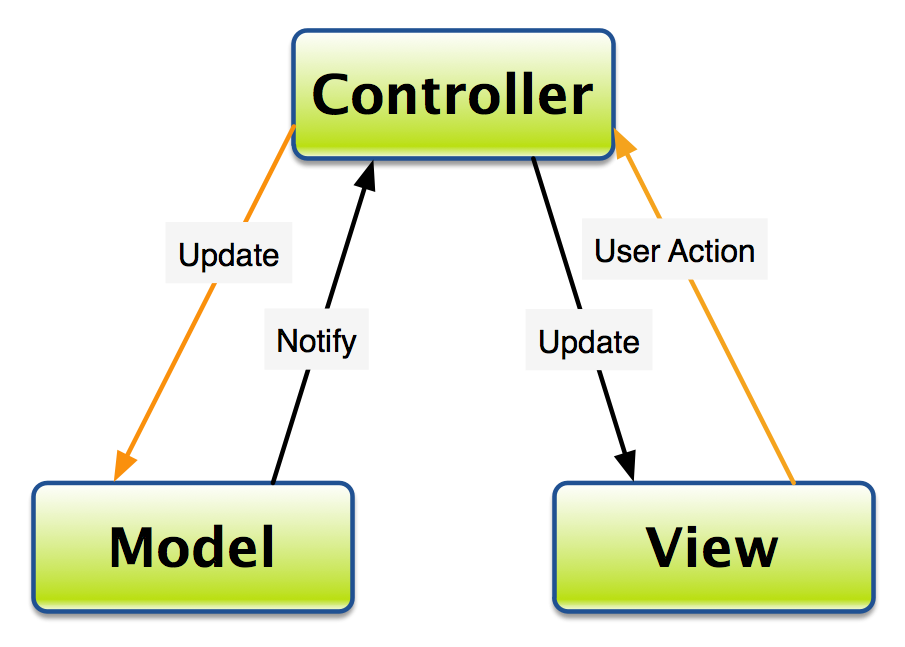
\includegraphics[width=0.5\textwidth]{Images/mvcPattern.png}
    \caption{\label{pic:mvc-pattern} Pattern MVC.}
\end{wrapfigure}

L'organizzazione del codice fatta in questo modo ci ha permesso di attribuire chiare responsabilità ad ognuno dei componenti, rendendoli indipendenti tra loro, facilmente integrabili e manutenibili. \newline \newline L'immagine \ref{pic:mvc-pattern} mostra l'architettura del pattern MVC. Il componente cuore è il \textit{controller} che ha i riferimenti sia del model che della view. Quest'ultimo avrà quindi modo di recuperare ed aggiornare i dati nel model, preparandoli e comunicandoli alla view. \newline \newline Viceversa quando l'utente interagisce con essa, la view richiama il controller per soddisfare la richiesta dell'utente. \newline \newline Il recupero ed il salvataggio dei dati nel model avviene tramite servizi che mettono a disposizione chiamate Http REST e l'interrogazione della suite di Azure. Per sfruttare i benefici del pattern MVC e mantenere una singola istanza per ciascuna componente (pattern Singleton) abbiamo dovuto confrontarci con framework che nativamente non sono predisposti a tale scopo.

\subsection{MVC e Windows Form}

Nelle applicazioni \textit{Windows Form} abbiamo utilizzato le classi \textit{Program.cs} come entry point delle applicazioni, ed in queste vengono avviati i vari controller che si occupano di creare e visualizzare le \textit{Forms} passandogli il proprio riferimento. I controller comunicano con l'entry point attraverso l'uso di funzioni passate dalla classe principale ai controller per mezzo del costruttore.

\subsection{MVC e Unity Platform}
Per quanto riguarda la piattaforma Unity, siamo riusciti ad applicare l'MVC creando degli oggetti rappresentanti le varie componenti del pattern. In questo modo le componenti si sono legate al life cycle della piattaforma Unity, permettendoci di applicare il pattern Singleton. Anche in questo caso \textit{Application} istanzia i vari controller che hanno il riferimento delle views e dei models. Le views hanno il riferimento del controllers per poter comunicare le interazioni dell'utente, mentre i controllers comunicano ad \textit{Application} tramite l'utilizzo di funzioni passate da questa ai controller per mezzo del costruttore. \newline \newline All'avvio di \textit{VitalSignsMonitorController}, questo esegue un servizio in background che si mette in ascolto dei messaggi di SignalR per un determinato digital twin.

\section{Organizzazione del Codice}

Il progetto è consultabile al seguente \href{https://github.com/lucagiorgettismp/AzureHealthcareDigitalTwins}{\textit{repository}} di GitHub. Il repository è organizzato nelle seguenti directory:

\begin{itemize}

    \item \textbf{HealthcareVitalSignsMonitor}: contiene la soluzione C\# del simulatore e del client;
    
    \item \textbf{DTDLModels}: contiene i file \texttt{.json} che rappresentano i modelli per la definizione dei digital twins;
    
    \item \textbf{AzureAppFunctions}: contiene la soluzione C\# di tutte le Azure function implementate;

    \item \textbf{HealthcareHololensClient}: contiene il progetto Unity per la parte di mixed reality;
        
    \item \textbf{doc}: contiene la documentazione in formato \texttt{.latex} e \texttt{.pdf}.
\end{itemize}

\subsection{Healthcare Vital Signs Monitor}
E' una solution .NET scritta in C\# che contiene tre progetti:
\begin{itemize}
    \item \textbf{Client} \newline
    Permette all'operatore di creare la scheda del paziente, al salvataggio della quale avviene la creazione del digital twin di questo, del monitor a parametri vitali e la creazione del device su IoTHub.
    \item \textbf{Simulator} \newline 
    Simula il funzionamento dell'asset fisico. Permette di selezionare su quale digital twin del monitor a parametri vitali emettere i valori, settare le soglie di allarme, i range dei valori e le unità di misura. 
    \newline Una volta selezionato il device, è possibile avviare il simulatore vero e proprio, che a ogni iterazione genera dei nuovi valori dei parametri. I nuovi valori sono quelli ottenuti dall'iterazione precedente, spostati in positivo o in negativo di un valore compreso in un range che va da \textit{+delta} a \textit{-delta}, dove \textit{delta} è una soglia preimpostata per il parametro; 
    \item \textbf{Common} \newline 
    Viene referenziato da entrambi i progetti precedentemente citati e contiene le classi condivise.
\end{itemize}

\subsection{Azure Digital Twins}

\subsubsection{Modelli}
In questa directory sono contenuti i modelli che permettono di definire le proprietà e che costituiscono lo stato dei digital twins. Questa fase è stata una delle prime, di tutte quelle di analisi, e ci ha aiutato a capire come poter meglio modellare successivamente i digital twins. \newline \newline I modelli vengono definiti usando il linguaggio \href{https://github.com/Azure/opendigitaltwins-dtdl/blob/master/DTDL/v2/dtdlv2.md}{DTDL} (Digital Twins Definition Language). Si possono utilizzare diverse strutture e tipi di dati a seconda del contesto di utilizzo e da cosa si deve andare a modellare: noi abbiamo utilizzato prevalentemente \textit{Property}, \textit{Object} e \textit{Component}. Le prime descrivono lo stato in lettura e scrittura di un digital twin. L'\textit{Object} è un tipo di dato composto da campi (simile ad un oggetto in OOP). I \textit{Components} possono essere considerati come delle interfacce che permettono di descrivere \textit{Property} utilizzate da altri modelli che utilizzeranno questa interfaccia. Il risultato della modellazione ha portato a creare un modello con \textit{Property} comuni (\textit{Base Param Content}), un modello per ogni sensore, uno per il monitor a parametri vitali e infine quello per la modellazione del paziente.  L'immagine \ref{pic:model-graph} mostra il grafo dei modelli e le loro relazioni. \newline \newline \newline \begin{figure}[ht]
    \includegraphics[width=14cm]{Images/ModelGraph.PNG}
    \centering
    \caption{\label{pic:model-graph}Grafo dei modelli.}
\end{figure}
Il significato delle frecce è il seguente:
\begin{itemize}
    \item la freccia verde indica una ereditarietà: ogni modello di un sensore eredita le proprietà comuni dal modello base;
    
    \item la freccia blu indica che ogni modello di un sensore è un \textit{Component} del modello del monitor a parametri vitali;
    
    \item la freccia gialla indica una relazione tra il modello del monitor e quello del paziente.
\end{itemize}

\subsubsection{Modello di Base (Base Param Content)}
Questo modello contiene le proprietà comuni ereditate da tutti gli altri modelli che rappresentano un sensore (parametri vitali e batteria). Nel frammento \ref{lst:model-graph} è presente una parte del corpo del modello. Contestualizziamo il \texttt{json} per chi non conosce il linguaggio DTDL, descrivendo alcune \textit{keyword}: con \texttt{@type} si indica il tipo di dato a cui appartiene un elemento del modello (ad esempio \textit{Property} o \textit{Object}) con \texttt{name} si indica l'id con cui identificare un elemento e con \texttt{schema} il tipo di dato di quel elemento (ad esempio se è un intero, double o stringa).
\begin{lstlisting}[label={lst:model-graph}, caption={Proprietà comuni del modello Base Param Content ereditate dai modelli.}, language=json, firstnumber=1]
 {
    "@type": "Property",
    "name": "sensor_value",
    "displayName": "Sensor value",
    "schema": {
      "@type": "Object",
      "fields": [
        {
          "name": "value",
          "displayName": "Value",
          "schema": "double"
        },
        {
          "name": "min_value",
          "displayName": "Min value",
          "schema": "double"
        },
          {
          "name": "max_value",
          "displayName": "Max value",
          "schema": "double"
        },
        {
          "name": "unit",
          "displayName": "Unit of measurement",
          "schema": "string"
        },
        {
          "name": "type",
          "displayName": "Value type",
          "schema": "string"
        }
      ]
    }
  }
\end{lstlisting}
Nel frammento di codice mostrato è definito un \textit{Object} i cui campi sono le proprietà ereditate. I campi modellati sono: il valore corrente del sensore, il valore minimo e massimo del sensore per essere considerato nella norma, l'unità di misura e il tipo di dato (nell'immagine con \texttt{name} type) a cui appartiene il valore corrente. 

\subsubsection{Modello di ogni Sensore}
Tutte le proprietà che non sono comuni ai sensori, e che quindi non possono ereditate dal modello base, sono contenute nei singoli modelli. Un' esempio è l'informazione del colore che i grafici e il valore puntuale del sensore devono assumere. Tale informazione, non presente nel sensore della batteria, è una stringa che rappresenta una tupla e contiene tre interi che rappresentano rispettivamente il canale del modello colore RGB.

\subsubsection{Modello del Monitor a Parametri Vitali}

Nel modello del monitor a parametri vitali è stato definito un \textit{Component} per ogni sensore. Il frammento \ref{lst:component-monitor-model} illustra la dichiarazione del \textit{Component} relativo alla temperatura. Per brevità si è deciso di mostrarne solamente uno ma è esteso a tutti gli altri sensori.
\begin{lstlisting}[label={lst:component-monitor-model}, caption={Componente temperature del modello del monitor.}, language=json, firstnumber=1]
    {
      "@type": "Component",
      "name": "temperature",
      "displayName": "Temperature Sensor",
      "schema": "dtmi:healthCareDT:TemperatureParam;1"
    }
\end{lstlisting}

Oltre ai \textit{Components}, vi sono due \textit{Property} di fondamentale importanza da descrivere:

\begin{itemize}
    \item \textit{device\_id}: identifica l'id univoco (che coincide con il codice fiscale del paziente) del dispositivo IoT nel Hub IoT precedentemente descritto. In questo modo si permette ai diversi clients Hololens di rimanere in ascolto in attesa di ricevere dei messaggi aventi questo id;
    
    \item \textit{last\_selected\_view}: permette di tenere traccia dell'ultimo pannello aperto in un client Hololens attraverso un intero. In questo modo alla riapertura dell'ologramma verrà visualizzato sempre quel pannello. Si tratta di una personalizzazione che abbiamo voluto realizzare in modo da rendere più agevole la visualizzazione dell'ologramma.
\end{itemize}

Infine, l'ultimo elemento è la relazione che lega i modelli (e quindi i digital twins) del monitor a parametri vitali e quello del paziente.
Il frammento \ref{lst:relation-monitor-model} illustra la sua definizione. Il significato di questa relazione è quello di stabilire che ogni paziente ha un solo monitor a parametri vitali di riferimento.

\begin{lstlisting}[label={lst:relation-monitor-model}, caption={Relazione del modello del monitor e quello del paziente.}, language=json, firstnumber=1]
    {
      "@type": "Relationship",
      "@id": "dtmi:healthCareDT:VitalParametersMonitor:rel_has_monitor;1",
      "name": "rel_has_monitor",
      "displayName": "Patient has a monitor",
      "target": "dtmi:healthCareDT:Patient;1"
    }
\end{lstlisting}

Nei campi \texttt{@id} e \texttt{target} si specificano gli id dei modelli coinvolti nella relazione.

\subsubsection{Modello del Paziente}
In questo modello sono contenute tutte le \textit{Property} relative alle informazioni che costituiscono la cartella clinica di un paziente come descritto nel capitolo \ref{chap:architectural-design} nella sezione dedicata al simulatore e a Hololens. \newline \newline Dove si è potuto, si sono utilizzati i \textit{Semantic Types}: insieme di tipi semantici che possono essere applicati a delle proprietà per caratterizzarle. Ad esempio per l'altezza e peso di un paziente si è utilizzato rispettivamente il tipo semantico \texttt{Length} (\(m\)) e \texttt{Mass} (\(Kg\)). L'indice di massa corporea, la cui unità di misura è \(Kg/m^2\), non ha un tipo semantico supportato. Per questo motivo si è creata una specifica proprietà che modella questa informazione.

\subsubsection{Azure function}
In questa sezione non ci sono particolari scelte implementative da evidenziare. Come già detto, l'obbiettivo delle Azure functions è quello di propagare nuove informazioni relative ai sensori e ai pazienti a componenti dell'architettura. I componenti coinvolti sono: 

\begin{itemize}
    \item IoT Hub \to \> istanza dei digital twins: per aggiornate lo stato dei digital twins a partire dai dati ricevuti dall'hub;
    
    \item Digital twins \to \> client Hololens: per far si che i client (Hololens, nel nostro caso) possano ricevere i nuovi dati per mezzo della libreria SignalR;
    
    \item Digital twins \to \> Time Series Insight: per permettere la persistenza dei dati in questo componente.
\end{itemize}

Quando vengono aggiornati i dati dai devices creati nel IoTHub, vengono eseguiti degli eventi che chiamano le funzioni create e aggiornano il digital twin di quel device e inviano un messaggio tramite SignalR. All'aggiornamento del digital twin, un altro evento permette di inviare uno snapshot del digital twin aggiornato a Time Series Insight.
In ciascuna funzione si sono quindi implementate le operazioni di parsing che analizzano il contenuto dei dati ricevuto in input, per poi propagarle al destinatario della funzione. \newline \newline La directory \textit{Model} contiene le classi POCO che modellano tutti i payload che le diverse Azure functions inviano ai rispettivi destinatari, permettendo di serializzare e deserializzare i messaggi rapidamente.

\subsection{Healthcare Hololens Client}

L'applicazione per client Hololens sviluppata ha un funzionamento che si divide in due fasi:
\begin{itemize}
    \item La lettura del QR code del paziente, il quale contiene il riferimento del proprio device di Azure;
    \item La visualizzazione del monitor a parametri vitali con la possibilità di selezionare diverse modalità di visualizzazione dei parametri.
\end{itemize}

L'entry point dell'applicazione è lo script \textit{Application.cs}, che gestisce il passaggio da una fase all'altra, istanziando due differenti controller:
\begin{itemize}
    \item \textbf{QRCodeController}: avvia il servizio background di rilevazione del QR code e prende in input una funzione da invocare non appena il QR code viene letto;
    
    \item \textbf{VitalSignsMonitorController}: una volta ottenuto l'id del device, recupera i dati del paziente\footnotemark{}, la schermata selezionata in precedenza e avvia il servizio di ascolto dei messaggi provenienti da SignalR. Al cambio della schermata notifica il pannello selezionato al server\footnotemark[\value{footnote}].
\end{itemize}

Tutte le classi contenute all'iterno alla cartella \textit{/View} degli script estendono \textit{MonoBeahaviour} e sono collegate al relativo elemento UI, così come lo sono i controller e \textit{Application.cs}.\\

La cartella \textit{/Model} contiene le classi POCO per la serializzazione e deserializzazione dei messaggi SignalR e verso il server, mentre nella cartella \textit{/Api} si trovano le classi per l'interazione con il database realtime di Firebase e per interrogare ed autenticarsi presso la suite di Azure.


\footnotetext{
    \textbf{Importante}: la libreria \textit{DigitalTwinClient} per l'autenticazione e l'interfacciamento con i Digital Twins di \textit{Azure} non funziona a \textit{runtime} su \textit{Hololens} (per mancanza di permessi di accesso ad una cartella privata del file system). \newline Per aggirare questo problema, il salvataggio del paziente e dell'ultima schermata aperta è stato replicato anche su Firebase RealTime Database.
    }
